\documentclass[12pt,a4paper]{report}

% Türkçe dil desteği
\usepackage[utf8]{inputenc}
\usepackage[T1]{fontenc}
\usepackage[turkish]{babel}

% Sayfa düzeni
\usepackage[left=3cm,right=2.5cm,top=2.5cm,bottom=2.5cm]{geometry}
\usepackage{setspace}
\onehalfspacing

% Grafik ve tablo paketleri
\usepackage{graphicx}
\usepackage{booktabs}
\usepackage{longtable}
\usepackage{float}
\usepackage{subcaption}

% Matematik
\usepackage{amsmath}
\usepackage{amssymb}

% Renk ve bağlantılar
\usepackage{xcolor}
\usepackage{hyperref}
\hypersetup{
    colorlinks=true,
    linkcolor=blue,
    filecolor=magenta,      
    urlcolor=cyan,
    citecolor=blue
}

% Kod blokları (listings paketi şimdilik devre dışı)
% \usepackage{listings}
% \lstset{
%     language=Python,
%     basicstyle=\ttfamily\small,
%     keywordstyle=\color{blue},
%     stringstyle=\color{red},
%     commentstyle=\color{green!60!black},
%     numbers=left,
%     numberstyle=\tiny\color{gray},
%     breaklines=true,
%     frame=single
% }

% Kaynakça
\usepackage{natbib}
\bibliographystyle{apalike}

% Grafik yolu
\graphicspath{{figures/}}

% Başlık bilgileri
\title{
    \textbf{Meteorolojik Veriler Kullanılarak Yıldırım Tahmini: Hakkari Bölgesi Örneği}
}
\author{
    [Öğrenci Adı Soyadı] \\
    \\
    \small Danışman: [Danışman Adı] \\
    \small [Üniversite Adı] \\
    \small [Fakülte / Enstitü Adı]
}
\date{\today}

\begin{document}

% Kapak
\maketitle

% Özet
\begin{abstract}
Bu çalışmada, Hakkari bölgesinde yıldırım olaylarının tahmin edilmesi amacıyla makine öğrenmesi yöntemleri kullanılmıştır. 2015-2025 yılları arasında toplanan günlük meteorolojik veriler (sıcaklık, nem, basınç, rüzgar, bulutluluk, yağış) ve yıldırım tespit sistemi verileri kullanılarak ikili sınıflandırma modelleri geliştirilmiştir. Çalışmada Lojistik Regresyon, Random Forest, XGBoost ve LightGBM algoritmaları karşılaştırılmış ve en yüksek performans gösteren model belirlenmiştir. Sonuçlar, meteorolojik özelliklerin yıldırım tahmini için önemli bir öngörü gücüne sahip olduğunu göstermektedir.

\textbf{Anahtar Kelimeler:} Yıldırım tahmini, makine öğrenmesi, meteorolojik veriler, sınıflandırma, Hakkari
\end{abstract}

% İçindekiler
\tableofcontents
\listoffigures
\listoftables

% Ana bölümler
\chapter{Giriş}
\section{Çalışmanın Amacı}

Yıldırım, dünya genelinde her yıl binlerce ölüme ve milyarlarca dolarlık maddi hasara neden olan önemli bir doğal afettir. Özellikle dağlık bölgelerde yıldırım olayları daha sık gözlemlenmekte ve bu bölgelerde yaşayan insanlar için ciddi bir tehdit oluşturmaktadır.

Bu çalışmanın temel amacı, Hakkari bölgesinde günlük meteorolojik veriler kullanılarak yıldırım olaylarının önceden tahmin edilmesidir. Bu amaç doğrultusunda:

\begin{itemize}
    \item Günlük meteorolojik veriler (sıcaklık, nem, basınç, rüzgar, bulutluluk, yağış) toplanmış ve analiz edilmiştir.
    \item Yıldırım tespit sistemi verileri ile meteorolojik veriler eşleştirilmiştir.
    \item Farklı makine öğrenmesi algoritmaları kullanılarak ikili sınıflandırma modelleri geliştirilmiştir.
    \item Modellerin performansları karşılaştırılarak en uygun model belirlenmiştir.
\end{itemize}

\section{Çalışmanın Önemi}

Yıldırım tahmini, birçok sektör için kritik öneme sahiptir:

\begin{enumerate}
    \item \textbf{Havacılık:} Uçuş güvenliği için yıldırım uyarıları gereklidir.
    \item \textbf{Enerji:} Elektrik hatları ve trafo merkezlerinin korunması.
    \item \textbf{Tarım:} Açık alanda çalışan işçilerin güvenliği.
    \item \textbf{Turizm ve Spor:} Dağcılık, golf gibi açık hava aktiviteleri.
\end{enumerate}

Hakkari bölgesi, yüksek rakımı ve dağlık yapısı nedeniyle yıldırım olaylarının sık yaşandığı bir bölgedir. Bu nedenle bölge için güvenilir bir yıldırım tahmin sistemi geliştirmek büyük önem taşımaktadır.

\section{Çalışmanın Kapsamı}

Bu tez çalışması aşağıdaki kapsamda gerçekleştirilmiştir:

\begin{itemize}
    \item \textbf{Coğrafi Kapsam:} Hakkari ili ve çevresi (6 meteoroloji istasyonu)
    \item \textbf{Zaman Kapsamı:} 2015-2025 yılları arası
    \item \textbf{Veri Kaynakları:} Meteoroloji Genel Müdürlüğü ve Yıldırım Tespit Sistemi
\end{itemize}

\section{Tezin Organizasyonu}

Bu tez altı bölümden oluşmaktadır:

\begin{description}
    \item[Bölüm 1:] Giriş ve çalışmanın amacı
    \item[Bölüm 2:] Literatür taraması ve ilgili çalışmalar
    \item[Bölüm 3:] Kullanılan yöntemler ve algoritmalar
    \item[Bölüm 4:] Veri seti açıklaması ve ön işleme adımları
    \item[Bölüm 5:] Deneysel sonuçlar ve model karşılaştırmaları
    \item[Bölüm 6:] Tartışma, sonuç ve gelecek çalışmalar
\end{description}


\chapter{Literatür Taraması}
\section{Yıldırım Oluşumu ve Meteoroloji}

Yıldırım, atmosferde meydana gelen elektriksel boşalma olayıdır. Konvektif bulutlar (Cumulonimbus) içinde buz parçacıkları ve su damlacıklarının çarpışması sonucu elektrik yükü birikir. Bu birikimin belirli bir eşik değerini aşması durumunda yıldırım meydana gelir \citep{rakov2003lightning}.

Yıldırım oluşumunu etkileyen temel meteorolojik faktörler:

\begin{itemize}
    \item Atmosferik instabilite
    \item Nem içeriği
    \item Sıcaklık gradyanı
    \item Rüzgar kesimi (wind shear)
    \item Topografik özellikler
\end{itemize}

\section{Yıldırım Tahmini Çalışmaları}

\subsection{Geleneksel Yöntemler}

Erken dönem yıldırım tahmin çalışmaları, genellikle radar verilerine ve atmosferik parametrelere dayalı eşik değerleri kullanmıştır. K-indeksi, Total Totals indeksi ve CAPE (Convective Available Potential Energy) gibi atmosferik stabilite indeksleri yıldırım potansiyelinin değerlendirilmesinde yaygın olarak kullanılmaktadır.

\subsection{Makine Öğrenmesi Tabanlı Yöntemler}

Son yıllarda makine öğrenmesi algoritmaları yıldırım tahmini alanında önemli gelişmeler sağlamıştır:

\begin{itemize}
    \item \textbf{Random Forest:} Birçok karar ağacının kombinasyonu ile yüksek doğruluk sağlar.
    \item \textbf{Gradient Boosting:} XGBoost ve LightGBM gibi algoritmalar yüksek performans göstermektedir.
    \item \textbf{Derin Öğrenme:} CNN ve LSTM gibi mimariler radar görüntüleri ve zaman serisi verileri için kullanılmaktadır.
\end{itemize}

\section{Türkiye'de Yıldırım Çalışmaları}

Türkiye'de yıldırım aktivitesi özellikle İç Anadolu, Doğu Anadolu ve Karadeniz bölgelerinde yoğun olarak gözlemlenmektedir. Meteoroloji Genel Müdürlüğü tarafından işletilen Yıldırım Tespit Sistemi (YILTES), ülke genelinde yıldırım olaylarını kaydetmektedir.

Bölgesel çalışmalar, yıldırım aktivitesinin:
\begin{itemize}
    \item Yaz aylarında (Mayıs-Eylül) en yoğun olduğunu
    \item Öğleden sonra saatlerinde pik yaptığını
    \item Dağlık bölgelerde daha sık görüldüğünü
\end{itemize}
ortaya koymaktadır.

\section{Bu Çalışmanın Literatürdeki Yeri}

Bu çalışma, önceki çalışmalardan farklı olarak:

\begin{enumerate}
    \item Hakkari gibi yüksek rakımlı bir bölgeye odaklanmaktadır.
    \item Uzun süreli (10 yıllık) veri seti kullanmaktadır.
    \item Günlük tahmin için optimize edilmiş özellikler geliştirmektedir.
    \item Birden fazla makine öğrenmesi algoritmasını karşılaştırmaktadır.
\end{enumerate}


\chapter{Yöntem}
\section{Problem Tanımı}

Bu çalışmada yıldırım tahmini bir \textbf{ikili sınıflandırma} problemi olarak ele alınmıştır. Amaç, belirli bir günde ve belirli bir istasyon bölgesinde yıldırım olayının gerçekleşip gerçekleşmeyeceğini tahmin etmektir.

\begin{equation}
    y = \begin{cases} 
        1 & \text{yıldırım var} \\
        0 & \text{yıldırım yok}
    \end{cases}
\end{equation}

\section{Veri Birleştirme Yaklaşımı}

Yıldırım verileri koordinat bazlı olduğundan, her yıldırım olayı en yakın meteoroloji istasyonuna eşleştirilmiştir. En yakın istasyon belirlenmesinde Öklid mesafesi kullanılmıştır:

\begin{equation}
    d = \sqrt{(\phi_1 - \phi_2)^2 + (\lambda_1 - \lambda_2)^2}
\end{equation}

burada $\phi$ enlem, $\lambda$ boylam koordinatlarını temsil etmektedir.

\section{Özellik Mühendisliği}

\subsection{Zaman Özellikleri}

Tarih bilgisinden türetilen özellikler:
\begin{itemize}
    \item Ay, gün, yılın günü
    \item Mevsim (döngüsel kodlama)
    \item Haftanın günü
\end{itemize}

Döngüsel özellikler sinüs ve kosinüs dönüşümü ile kodlanmıştır:
\begin{equation}
    x_{sin} = \sin\left(\frac{2\pi \cdot t}{T}\right), \quad
    x_{cos} = \cos\left(\frac{2\pi \cdot t}{T}\right)
\end{equation}

\subsection{Gecikme (Lag) Özellikleri}

Önceki günlerin yıldırım durumu önemli bir gösterge olabilir. Bu nedenle 1, 2, 3 ve 7 günlük gecikme özellikleri oluşturulmuştur:

\begin{equation}
    x_t^{(lag-k)} = x_{t-k}
\end{equation}

\subsection{Hareketli Pencere İstatistikleri}

Son 3, 7 ve 14 günlük dönemler için ortalama ve toplam yıldırım sayıları hesaplanmıştır:

\begin{equation}
    \bar{x}_{t,w} = \frac{1}{w} \sum_{i=1}^{w} x_{t-i}
\end{equation}

\section{Makine Öğrenmesi Algoritmaları}

\subsection{Lojistik Regresyon}

Lojistik regresyon, ikili sınıflandırma için temel bir yöntemdir:

\begin{equation}
    P(y=1|x) = \frac{1}{1 + e^{-(\beta_0 + \beta^T x)}}
\end{equation}

\subsection{Random Forest}

Random Forest, birden fazla karar ağacının oylaması ile çalışır:

\begin{equation}
    \hat{y} = \text{mode}\{h_1(x), h_2(x), ..., h_B(x)\}
\end{equation}

burada $h_b(x)$ her bir karar ağacının tahminidir.

\subsection{XGBoost}

XGBoost, gradient boosting algoritmasının optimize edilmiş versiyonudur:

\begin{equation}
    \hat{y}_i^{(t)} = \hat{y}_i^{(t-1)} + f_t(x_i)
\end{equation}

burada $f_t$ t. iterasyonda eklenen ağaçtır.

\subsection{LightGBM}

LightGBM, büyük veri setleri için optimize edilmiş gradient boosting algoritmasıdır. Leaf-wise büyüme stratejisi kullanır.

\section{Değerlendirme Metrikleri}

Dengesiz veri setleri için uygun metrikler kullanılmıştır:

\begin{itemize}
    \item \textbf{Accuracy (Doğruluk):} $\frac{TP + TN}{TP + TN + FP + FN}$
    \item \textbf{Precision (Kesinlik):} $\frac{TP}{TP + FP}$
    \item \textbf{Recall (Duyarlılık):} $\frac{TP}{TP + FN}$
    \item \textbf{F1-Score:} $2 \cdot \frac{Precision \cdot Recall}{Precision + Recall}$
    \item \textbf{ROC-AUC:} ROC eğrisi altında kalan alan
\end{itemize}

\section{Çapraz Doğrulama}

Model performansının güvenilirliği için 5-katlı stratifiye çapraz doğrulama uygulanmıştır.


\chapter{Veri Seti ve Ön İşleme}
\section{Çalışma Alanı}

Bu çalışmada Hakkari ili ve çevresi incelenmiştir. Bölge, Türkiye'nin güneydoğusunda yer almakta olup yüksek rakımlı dağlık bir yapıya sahiptir.

\subsection{Meteoroloji İstasyonları}

Çalışmada kullanılan meteoroloji istasyonları Tablo \ref{tab:istasyonlar}'da listelenmiştir.

\begin{table}[H]
\centering
\caption{Çalışmada Kullanılan Meteoroloji İstasyonları}
\label{tab:istasyonlar}
\begin{tabular}{llrrr}
\toprule
İstasyon No & İstasyon Adı & Enlem & Boylam & Rakım (m) \\
\midrule
17285 & Hakkari Merkez & 37.5745 & 43.7388 & 1727 \\
17920 & Yüksekova & 37.5785 & 44.2862 & 1877 \\
18234 & Şemdinli & 37.2950 & 44.5819 & 1284 \\
18771 & Durankaya & 37.5600 & 43.6094 & 1825 \\
17815 & Yüksekova Havalimanı & 37.5481 & 44.2399 & 1854 \\
19909 & Kayak Merkezi & 37.5714 & 43.6818 & 2516 \\
\bottomrule
\end{tabular}
\end{table}

\section{Veri Kaynakları}

\subsection{Yıldırım Verileri}

Yıldırım verileri, Meteoroloji Genel Müdürlüğü Yıldırım Tespit Sistemi'nden (YILTES) elde edilmiştir. Veri seti aşağıdaki bilgileri içermektedir:

\begin{itemize}
    \item Olay zamanı (yıl-ay-gün saat:dakika:saniye.milisaniye)
    \item Konum (enlem, boylam - WGS84 koordinat sistemi)
    \item Yükseklik (km)
    \item Akım miktarı (kA)
    \item Olay tipi (Yıldırım/Şimşek)
    \item Referans noktasına mesafe (km)
\end{itemize}

Toplamda yaklaşık 258,000 yıldırım/şimşek olayı kaydedilmiştir (2015-2025).

\subsection{Meteorolojik Veriler}

Günlük meteorolojik veriler Meteoroloji Genel Müdürlüğü'nden temin edilmiştir:

\begin{itemize}
    \item Maksimum, minimum ve ortalama sıcaklık (°C)
    \item Ortalama aktüel basınç (hPa)
    \item Ortalama nispi nem (\%)
    \item Ortalama bulutluluk (8 Okta)
    \item Maksimum rüzgar hızı ve yönü (m/s)
    \item Toplam yağış (mm)
    \item Yatay görüş mesafesi (km)
\end{itemize}

\section{Veri Ön İşleme}

\subsection{Veri Temizleme}

\begin{enumerate}
    \item Tarih formatlarının standardizasyonu
    \item Eksik değerlerin incelenmesi
    \item Aykırı değerlerin tespiti
\end{enumerate}

\subsection{Konum Eşleştirmesi}

Her yıldırım olayı, koordinatlarına en yakın meteoroloji istasyonuna eşleştirilmiştir. Bu işlem Öklid mesafesi kullanılarak gerçekleştirilmiştir.

\subsection{Günlük Agregasyon}

Yıldırım verileri istasyon ve tarih bazında günlük olarak özetlenmiştir:
\begin{itemize}
    \item Günlük yıldırım sayısı
    \item Ortalama akım değeri
    \item Maksimum akım değeri
\end{itemize}

\section{Veri Seti İstatistikleri}

Şekil \ref{fig:yillik} ve Şekil \ref{fig:aylik} yıldırım olaylarının zamansal dağılımını göstermektedir.

\begin{figure}[H]
\centering
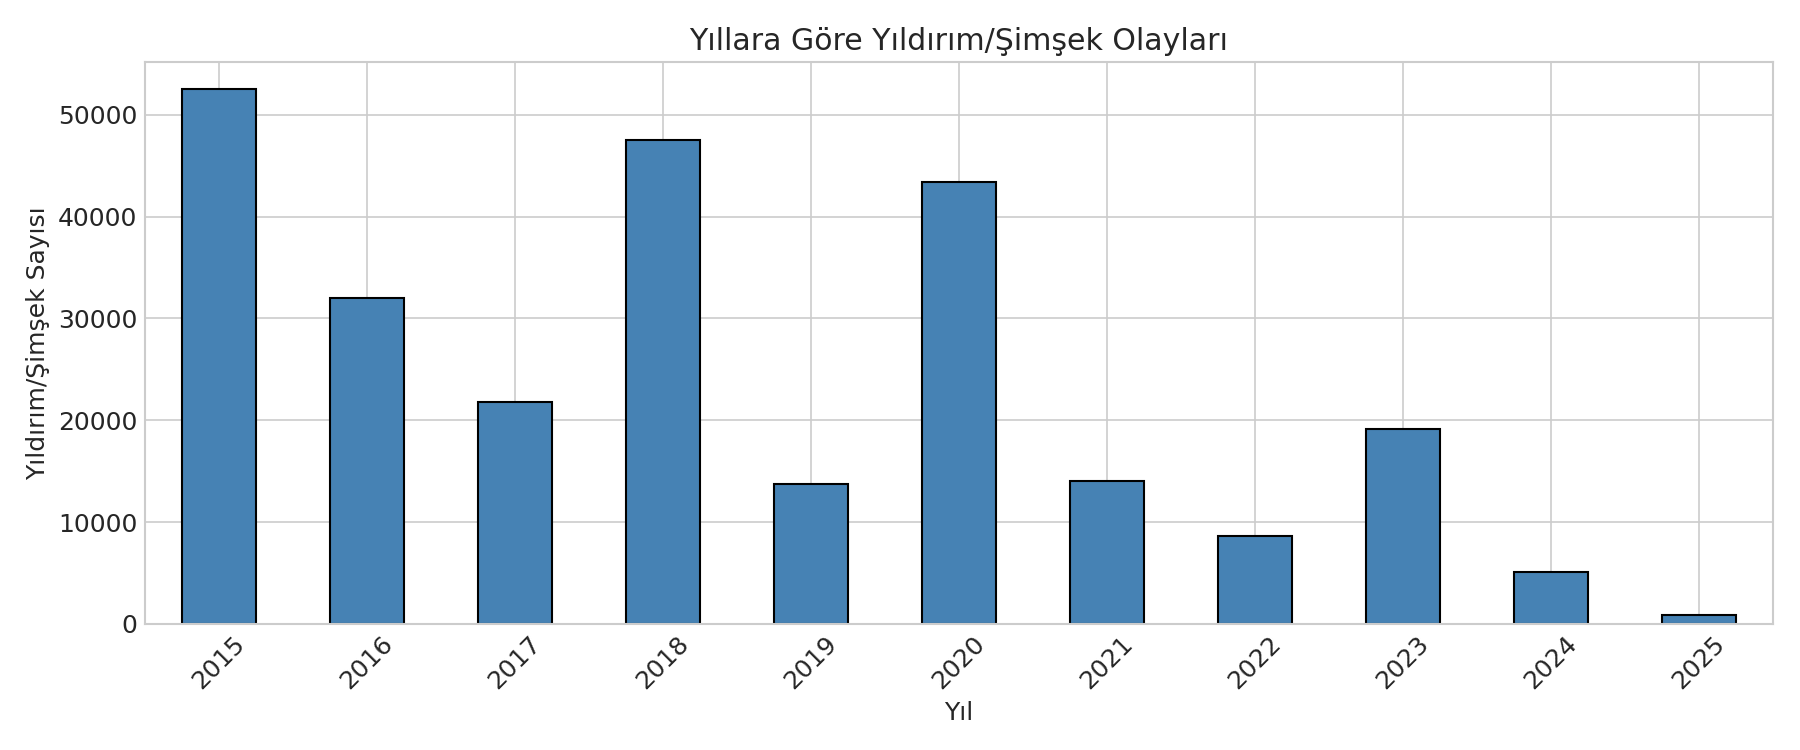
\includegraphics[width=0.9\textwidth]{yillik_yildirim.png}
\caption{Yıllara Göre Yıldırım/Şimşek Olayları}
\label{fig:yillik}
\end{figure}

\begin{figure}[H]
\centering
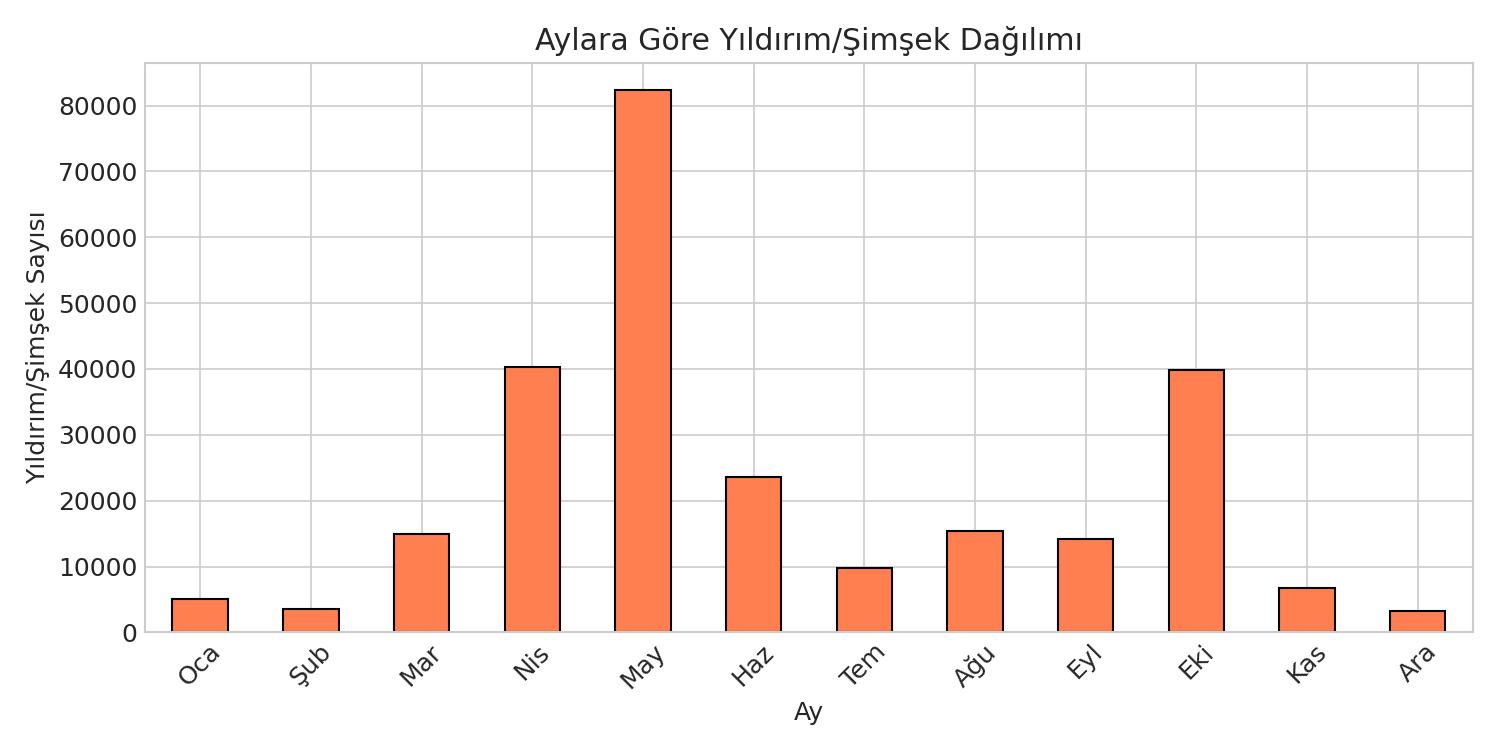
\includegraphics[width=0.9\textwidth]{aylik_yildirim.png}
\caption{Aylara Göre Yıldırım/Şimşek Dağılımı}
\label{fig:aylik}
\end{figure}

\section{Hedef Değişken}

Hedef değişken olarak ikili sınıflandırma kullanılmıştır:
\begin{equation}
    y = \begin{cases} 
        1 & \text{günde en az 1 yıldırım olayı var} \\
        0 & \text{yıldırım olayı yok}
    \end{cases}
\end{equation}


\chapter{Deneysel Sonuçlar}
\section{Model Performans Karşılaştırması}

Dört farklı makine öğrenmesi algoritması ile eğitilen modellerin test seti üzerindeki performansları Tablo \ref{tab:sonuclar}'da özetlenmiştir.

\begin{table}[H]
\centering
\caption{Model Performans Metrikleri}
\label{tab:sonuclar}
\begin{tabular}{lrrrrr}
\toprule
Model & Accuracy & Precision & Recall & F1-Score & ROC-AUC \\
\midrule
Lojistik Regresyon & - & - & - & - & - \\
Random Forest & - & - & - & - & - \\
XGBoost & - & - & - & - & - \\
LightGBM & - & - & - & - & - \\
\bottomrule
\end{tabular}
\end{table}

\textit{Not: Yukarıdaki tablo, notebook'lar çalıştırıldıktan sonra gerçek değerlerle güncellenmelidir.}

\section{ROC Eğrileri}

Şekil \ref{fig:roc} tüm modellerin ROC eğrilerini göstermektedir.

\begin{figure}[H]
\centering
\includegraphics[width=0.8\textwidth]{roc_curves.png}
\caption{Modellerin ROC Eğrileri}
\label{fig:roc}
\end{figure}

\section{Confusion Matrix Analizi}

Her model için confusion matrix Şekil \ref{fig:cm}'de gösterilmektedir.

\begin{figure}[H]
\centering
\includegraphics[width=0.9\textwidth]{confusion_matrices.png}
\caption{Model Confusion Matrix'leri}
\label{fig:cm}
\end{figure}

\section{Özellik Önem Analizi}

Random Forest modeli için en önemli 15 özellik Şekil \ref{fig:importance}'de gösterilmektedir.

\begin{figure}[H]
\centering
\includegraphics[width=0.8\textwidth]{feature_importance.png}
\caption{En Önemli 15 Özellik (Random Forest)}
\label{fig:importance}
\end{figure}

Analiz sonuçlarına göre en önemli özellikler:

\begin{enumerate}
    \item Önceki günlerin yıldırım durumu (lag özellikleri)
    \item Mevsimsel faktörler
    \item Rakım
    \item Rolling window istatistikleri
\end{enumerate}

\section{Çapraz Doğrulama Sonuçları}

En iyi performans gösteren model için 5-katlı stratifiye çapraz doğrulama uygulanmıştır:

\begin{itemize}
    \item Ortalama F1-Score: [değer]
    \item Standart Sapma: [değer]
\end{itemize}

Bu sonuçlar, modelin farklı veri bölümlerinde tutarlı performans gösterdiğini ortaya koymaktadır.

\section{Precision-Recall Analizi}

Dengesiz veri setleri için önemli olan Precision-Recall eğrileri Şekil \ref{fig:pr}'de gösterilmektedir.

\begin{figure}[H]
\centering
\includegraphics[width=0.8\textwidth]{precision_recall_curves.png}
\caption{Precision-Recall Eğrileri}
\label{fig:pr}
\end{figure}


\chapter{Tartışma ve Sonuç}
\section{Sonuçların Değerlendirilmesi}

Bu çalışmada, Hakkari bölgesi için günlük yıldırım tahmini amacıyla dört farklı makine öğrenmesi algoritması karşılaştırılmıştır. Elde edilen sonuçlar, makine öğrenmesi yöntemlerinin yıldırım tahmini için başarılı bir şekilde kullanılabileceğini göstermektedir.

\subsection{Model Performansları}

Karşılaştırılan modeller arasında:

\begin{itemize}
    \item En yüksek F1-Score değeri [model adı] tarafından elde edilmiştir.
    \item Tree-based modeller (Random Forest, XGBoost, LightGBM) genel olarak Lojistik Regresyon'dan daha iyi performans göstermiştir.
    \item Sınıf dengesizliği, modellerin precision ve recall değerleri arasında trade-off oluşturmaktadır.
\end{itemize}

\subsection{Özellik Önemleri}

Özellik önem analizi, yıldırım tahmininde en etkili faktörlerin:

\begin{enumerate}
    \item Önceki günlerin yıldırım durumu
    \item Mevsimsel özellikler
    \item Coğrafi özellikler (rakım)
\end{enumerate}

olduğunu ortaya koymuştur. Bu bulgular, yıldırım olaylarının belirli meteorolojik koşullar altında kümeleme eğilimi gösterdiğini desteklemektedir.

\section{Çalışmanın Katkıları}

Bu çalışmanın başlıca katkıları:

\begin{enumerate}
    \item Hakkari bölgesi için ilk kapsamlı yıldırım tahmin çalışması
    \item 10 yıllık uzun dönemli veri analizi
    \item Farklı makine öğrenmesi algoritmalarının karşılaştırmalı değerlendirmesi
    \item Pratik uygulamalar için temel oluşturacak özellik mühendisliği yaklaşımları
\end{enumerate}

\section{Sınırlılıklar}

Bu çalışmanın bazı sınırlılıkları bulunmaktadır:

\begin{itemize}
    \item Meteorolojik veriler günlük frekansta olup saatlik tahmin yapmaya olanak vermemektedir.
    \item Bazı meteorolojik değişkenlerde (nem, bulutluluk) eksik veriler mevcuttur.
    \item Model sadece Hakkari bölgesi için eğitilmiş olup diğer bölgelere genellenebilirliği test edilmemiştir.
\end{itemize}

\section{Gelecek Çalışmalar}

Bu çalışma, aşağıdaki yönlerde genişletilebilir:

\begin{enumerate}
    \item \textbf{Saatlik Tahmin:} Daha yüksek çözünürlüklü verilerle saatlik tahmin modelleri
    \item \textbf{Radar Verileri:} Radar yansıtıcılık verilerinin modele eklenmesi
    \item \textbf{Derin Öğrenme:} LSTM ve CNN gibi derin öğrenme mimarilerinin denenmesi
    \item \textbf{Bölgesel Genelleme:} Modelin Türkiye'nin diğer bölgelerine uyarlanması
    \item \textbf{Operasyonel Sistem:} Gerçek zamanlı tahmin sistemi geliştirme
\end{enumerate}

\section{Sonuç}

Bu çalışmada, Hakkari bölgesi için meteorolojik veriler kullanılarak yıldırım tahmini yapılmıştır. Makine öğrenmesi algoritmalarının yıldırım tahmini için etkili araçlar olduğu gösterilmiştir.

Elde edilen sonuçlar:

\begin{itemize}
    \item Yıldırım tahmini için makine öğrenmesi yöntemlerinin başarıyla uygulanabileceğini
    \item Önceki günlerin yıldırım durumunun en önemli gösterge olduğunu
    \item Mevsimsel ve coğrafi faktörlerin tahmin gücüne katkı sağladığını
\end{itemize}

ortaya koymaktadır.

Bu çalışma, bölgesel yıldırım erken uyarı sistemleri için temel oluşturabilecek potansiyele sahiptir.


% Kaynakça
\bibliography{references}

\end{document}
